\documentclass[journal,12pt,onecolumn]{IEEEtran}
\usepackage{cite}
\usepackage{amsmath,amssymb,amsfonts,amsthm}
\usepackage{algorithmic}
\usepackage{graphicx}
\usepackage{textcomp}
\usepackage{xcolor}
\usepackage{txfonts}
\usepackage{listings}
\usepackage{circuitikz}
\usepackage{enumitem}
\usepackage{mathtools}
\usepackage{gensymb}
\usepackage{comment}
\usepackage[breaklinks=true]{hyperref}
\usepackage{tkz-euclide} 
\usepackage{gvv}                                        
\usepackage[latin1]{inputenc}                                
\usepackage{color}                                            
\usepackage{array}                                            
\usepackage{longtable}                                       
\usepackage{calc}                                             
\usepackage{multirow}                                         
\usepackage{hhline}                                           
\usepackage{ifthen}                                           
\usepackage{lscape}
\usepackage{tabularx}
\usepackage{array}
\usepackage{float}
\usepackage{multicol}
\usepackage{caption}
\usetikzlibrary{patterns}

\newtheorem{theorem}{Theorem}[section]
\newtheorem{problem}{Problem}
\newtheorem{proposition}{Proposition}[section]
\newtheorem{lemma}{Lemma}[section]
\newtheorem{corollary}[theorem]{Corollary}
\newtheorem{example}{Example}[section]
\newtheorem{definition}[problem]{Definition}
\newcommand{\BEQA}{\begin{eqnarray}}
\newcommand{\EEQA}{\end{eqnarray}}
\newcommand{\define}{\stackrel{\triangle}{=}}
\theoremstyle{remark}
\newtheorem{rem}{Remark}

% Marks the beginning of the document
\begin{document}
\bibliographystyle{IEEEtran}
\vspace{3cm}

\title{Assignment 7}
\author{DESABOINA SRI SATHWIK-AI24BTECH11007}
\maketitle
% Removed \newpage to avoid a blank first page
\bigskip

\section*{GATE-2011:CE}

\begin{enumerate}
\item 
	 $[A]$ is a square matrix which is neither symmetric nor skew-symmetric and $[A]^\top$ is its transpose. The sum and difference of these matrices are defined as $[S] = [A] + [A]^\top$ and $[D] = [A] - [A]^\top$, respectively. Which of the following statements is TRUE?

		\hfill (CE:2011)
    
        \begin{enumerate}
            \item Both $[S]$ and $[D]$are symmetric
            \item Both $[S]$ and $[D]$ are skew-symmetric
            \item $[S]$ is skew-symmetric and $[D]$ is symmetric
            \item $[S]$ is symmetric and $[D]$ is skew-symmetric
        \end{enumerate}
\vspace{1cm}
    \item 
	    The square root of a number $N$ is to be obtained by applying the Newton Raphson iterations to the equation $x^2 - N = 0$. If $i$ denotes the iteration index, the correct iterative scheme will be

		\hfill (CE:2011)
    \begin{multicols}{2}
	    \begin{enumerate}
            \item $x_{i+1} = \frac{1}{2} \left( x_i + \frac{N}{x_i} \right)$
            \item $x_{i+1} = \frac{1}{2} \left( x_i^2 + \frac{N}{x_i^2} \right)$
            \item $x_{i+1} = \frac{1}{2} \left( x_i + \frac{N^2}{x_i} \right)$
            \item $x_{i+1} = \frac{1}{2} \left( x_i - \frac{N}{x_i} \right)$
        \end{enumerate}
    \end{multicols}

    \item
	    There are two containers, with one containing $4$ Red and $3$ Green balls and the other containing $3$ Blue and $4$ Green balls. One ball is drawn at random from each container. The probability that one of the balls is Red and the other is Blue will be

		\hfill (CE:2011)
    \begin{multicols}{4}
        \begin{enumerate}
            \item $1/7$
            \item $9/49$
            \item $12/49$
            \item $3/7$
        \end{enumerate}
    \end{multicols}

    \item
	    For the fillet weld of size '$s$' shown in the adjoining figure the effective throat thickness is
		\begin{center}
		

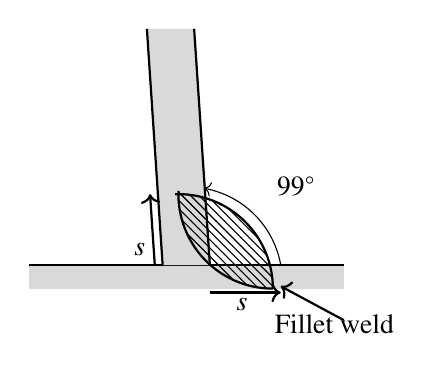
\begin{tikzpicture}

    % Draw the horizontal base plate
    \fill[gray!30] (-2,0) rectangle (2,-0.3); % Shaded base plate
    \draw[thick] (-2,0) -- (2,0);

    % Draw the vertical plate
    \fill[gray!30] (-0.3,0) -- (-0.5,3) -- (0.1,3) -- (0.3,0) -- cycle; % Shaded vertical plate
    \draw[thick] (-0.3,0) -- (-0.5,3); % Left side
    \draw[thick] (0.3,0) -- (0.1,3); % Right side
	\draw[thick][->] (-0.4,0) -- (-0.46,0.9);
	\draw[thick][->] (0.3,-0.35) -- (1.2,-0.35);
	\draw[thick][->] (2,-0.7) -- (1.2,-0.27);


    % Draw the fillet weld area
    \fill[pattern=north west lines] (1.1,-0.3) arc[start angle=0, end angle=92, radius=1.2cm] -- (1.1,-0.3);
    \draw[thick] (1.1,-0.3) arc[start angle=0, end angle=92, radius=1.2cm];
	\draw[thick] (1.1,-0.3) arc[start angle=270, end angle=178, radius=1.2cm]; \fill[pattern=north west lines] (1.1,-0.3) arc[start angle=270, end angle=178, radius=1.2cm] -- (1.1,-0.3);

    % Draw the angle label
    \draw[->] (1.2,0) arc[start angle=10, end angle=80, radius=1.2cm];
    \node at (1.4,1) {$99^\circ$};

    % Label 's' for the fillet weld throat thickness
    \node at (0.7,-0.5) {$s$};
    \node at (-0.6,0.2) {$s$};

    % Label for "Fillet weld"
    \node[below right] at (1,-0.5) {Fillet weld};

\end{tikzpicture}


		\end{center}

	    \hfill (CE:2011)
    \begin{multicols}{4}
        \begin{enumerate}
            \item $0.61 \, s$
            \item $0.65 \, s$
            \item $0.70 \, s$
            \item $0.75 \, s$
        \end{enumerate}
    \end{multicols}

    \item 
	    A $16$ mm thick plate measuring $650 \, \text{mm} \times 420 \, \text{mm}$ is used as a base plate for an ISHB $300$ column subjected to a factored axial compressive load of $2000$ kN. As per IS $456-2000$, the minimum grade of concrete that should be used below the base plate for safely carrying the load is 

		\hfill (CE:2011)
    \begin{multicols}{4}
        \begin{enumerate}
            \item $M15$
            \item $M20$
            \item $M30$
            \item $M40$
        \end{enumerate}
    \end{multicols} 
    
\item 
	Consider a reinforcing bar embedded in concrete. In a marine environment this bar undergoes uniform corrosion, which leads to the deposition of corrosion products on its surface and an increase in the apparent volume of the bar. This subjects the surrounding concrete to expansive pressure. As a result, corrosion induced cracks appear at the surface of concrete. Which of the following statements is TRUE? 

	\hfill (CE:2011)
        \begin{enumerate}
            \item Corrosion causes circumferential tensile stresses in concrete and the cracks will be parallel to the corroded reinforcing bar.
            \item Corrosion causes radial tensile stresses in concrete and the cracks will be parallel to the corroded reinforcing bar.
            \item Corrosion causes circumferential tensile stresses in concrete and the cracks will be perpendicular to the direction of the corroded reinforcing bar.
            \item Corrosion causes radial tensile stresses in concrete and the cracks will be perpendicular to the direction of the corroded reinforcing bar.
        \end{enumerate}

    \item 
	    The results for sieve analysis carried out for three types of sand, $P$, $Q$ and $R$, are given in the adjoining figure. If the fineness modulus values of the three sands are given as $FM_P$, $FM_Q$ and $FM_R$, it can be stated that

	    \begin{center}
    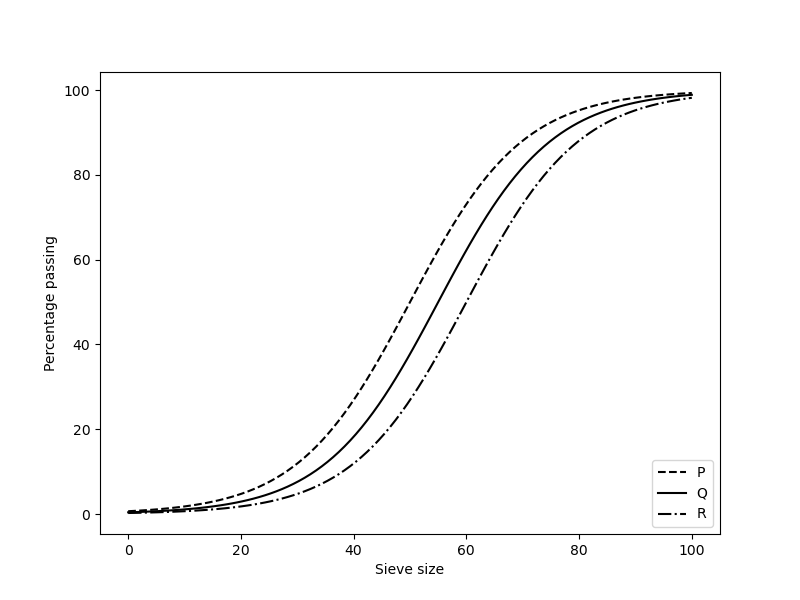
\includegraphics[width=0.5\textwidth]{figs/graph.png}
\end{center}
	    \hfill (CE:2011)
    \begin{multicols}{2}
        \begin{enumerate}
            \item \(FM_Q = \sqrt{FM_P \times FM_R}\)
            \item \(FM_Q = 0.5 \, (FM_P + FM_R)\)
            \item \(FM_P > FM_Q > FM_R\)
            \item \(FM_P < FM_Q < FM_R\)
        \end{enumerate}
    \end{multicols}
    
    \item 
	    The cross-section of a thermo-mechanically treated (TMT) reinforcing bar has

	    \hfill (CE:2011)
            \begin{enumerate}
            \item soft ferrite-pearlite throughout.
            \item hard martensite throughout.
            \item a soft ferrite-pearlite core with a hard martensitic rim.
            \item a hard martensitic core with a soft pearlite-bainitic rim.
        \end{enumerate}
    
    \item
	    Consider a simply supported beam with a uniformly distributed load having a neutral axis (NA) as shown. For points $P$ (on the neutral axis) and $Q$ (at the bottom of the beam) the state of stress is best represented by which of the following pairs? 

	    \begin{center}
		    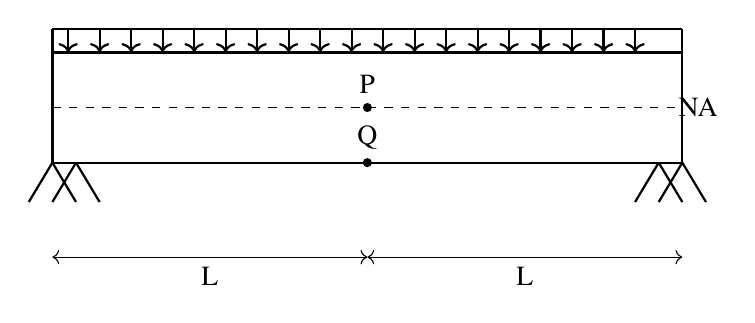
\begin{tikzpicture}

    % Beam
    \draw[thick] (-4,0) -- (4,0);
 \draw[thick] (-4,1.4) -- (4,1.4);
 \draw[thick] (-4,1.7) -- (4,1.7);
 \draw[thick] (-4,0) -- (-4,1.7);
 \draw[thick] (4,0) -- (4,1.7);


    % Supports
    \draw[thick] (-4,-0.5) -- (-3.7,0);
    \draw[thick] (-4.3,-0.5) -- (-4,0);
    \draw[thick] (4,-0.5) -- (3.7,0);
    \draw[thick] (4.3,-0.5) -- (4,0);
    \draw[thick] (3.7,-0.5) -- (4,0);
    \draw[thick] (3.4,-0.5) -- (3.7,0);
	\draw[thick] (-3.7,-0.5) -- (-4,0);
	\draw[thick] (-3.4,-0.5) -- (-3.7,0);

    % Distributed load
    \foreach \x in {-3.8,-3.4,...,3.8}
        \draw[thick,->] (\x,1.7) -- (\x,1.4);

    % Neutral Axis
    \draw[dashed] (-4,0.7) -- (4,0.7);
    \node at (4.2,0.7) {NA};

    % Points P and Q
    \draw[fill=black] (0,0.7) circle (0.05);
    \node[above] at (0,0.75) {P};
    \draw[fill=black] (0,0) circle (0.05);
    \node[above] at (0,0.05) {Q};

    % Dimensions
    \draw[<->] (-4,-1.2) -- (0,-1.2);
    \node[below] at (-2,-1.2) {L};
    \draw[<->] (0,-1.2) -- (4,-1.2);
    \node[below] at (2,-1.2) {L};

\end{tikzpicture}


	    \end{center}

	    \hfill {(CE:2011)}
	    \begin{multicols}{2}
        \begin{enumerate}
	    \item 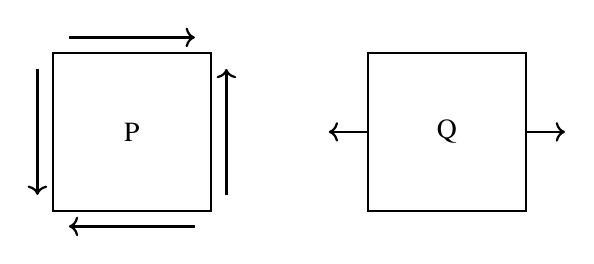
\begin{tikzpicture}

% Square P
\draw[thick] (0, 0) rectangle (2, 2);
\node at (1, 1) {P};

% Arrows around P
\draw[->, thick] (0.2, 2.2) -- (1.8, 2.2);
\draw[->, thick] (2.2, 0.2) -- (2.2, 1.8);
\draw[->, thick] (-0.2, 1.8) -- (-0.2, 0.2);
\draw[->, thick] (1.8, -0.2) -- (0.2, -0.2);

% Square Q
\draw[thick] (4, 0) rectangle (6, 2);
\node at (5, 1) {Q};

% Arrows around Q
\draw[<-, thick] (3.5, 1) -- (4, 1);
\draw[->, thick] (6, 1) -- (6.5, 1);

\end{tikzpicture}

	    \item 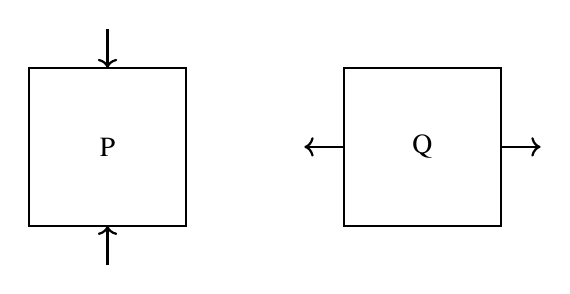
\begin{tikzpicture}

% Square P
\draw[thick] (0, 0) rectangle (2, 2);
\node at (1, 1) {P};

% Arrows around P
\draw[->, thick] (1,-0.5) -- (1, 0);
\draw[->, thick] (1, 2.5) -- (1, 2);


% Square Q
\draw[thick] (4, 0) rectangle (6, 2);
\node at (5, 1) {Q};

% Arrows around Q
\draw[<-, thick] (3.5, 1) -- (4, 1);
\draw[->, thick] (6, 1) -- (6.5, 1);

\end{tikzpicture}

 
	    \item 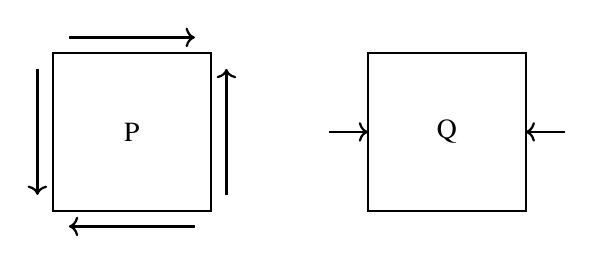
\begin{tikzpicture}

% Square P
\draw[thick] (0, 0) rectangle (2, 2);
\node at (1, 1) {P};

% Arrows around P
\draw[->, thick] (0.2, 2.2) -- (1.8, 2.2);
\draw[->, thick] (2.2, 0.2) -- (2.2, 1.8);
\draw[->, thick] (-0.2, 1.8) -- (-0.2, 0.2);
\draw[->, thick] (1.8, -0.2) -- (0.2, -0.2);

% Square Q
\draw[thick] (4, 0) rectangle (6, 2);
\node at (5, 1) {Q};

% Arrows around Q
\draw[->, thick] (3.5, 1) -- (4, 1);
\draw[<-, thick] (6, 1) -- (6.5, 1);

\end{tikzpicture}

 
	    \item 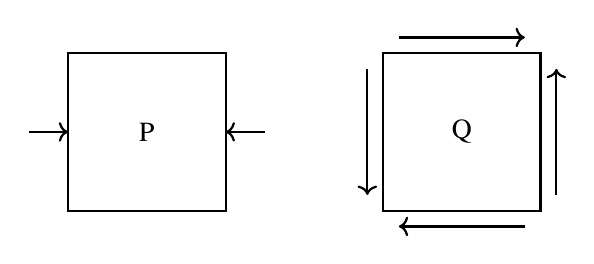
\begin{tikzpicture}

% Square P
\draw[thick] (0, 0) rectangle (2, 2);
\node at (1, 1) {P};

% Arrows around P
\draw[->, thick] (4.2, 2.2) -- (5.8, 2.2);
\draw[->, thick] (6.2, 0.2) -- (6.2, 1.8);
\draw[->, thick] (3.8, 1.8) -- (3.8, 0.2);
\draw[->, thick] (5.8, -0.2) -- (4.2, -0.2);

% Square Q
\draw[thick] (4, 0) rectangle (6, 2);
\node at (5, 1) {Q};

% Arrows around Q
\draw[->, thick] (-0.5, 1) -- (0, 1);
\draw[<-, thick] (2, 1) -- (2.5, 1);

\end{tikzpicture}

 
        \end{enumerate}
	    \end{multicols}
	    
\item For a saturated sand deposit, the void ratio and the specific gravity of solids are $0.70$ and $2.67$, respectively. The critical (upward) hydraulic gradient for the deposit would be

    \hfill{(CE:2011)}
    \begin{multicols}{4}
        \begin{enumerate}
            \item 0.54
            \item 0.98
            \item 1.02
            \item 1.87
        \end{enumerate}
    \end{multicols}
    \vspace{1cm}
    \item Likelihood of general shear failure for an isolated footing in sand decreases with

    \hfill{(CE:2011)}
        \begin{enumerate}
            \item decreasing footing depth
            \item decreasing inter-granular packing of the sand
            \item increasing footing width
            \item decreasing soil grain compressibility
        \end{enumerate}
\vspace{1cm}
    \item For a sample of dry, cohesionless soil with friction angle, $\phi$, the failure plane will be inclined to the major principal plane by an angle equal to

    \hfill{(CE:2011)}
    \begin{multicols}{4}
        \begin{enumerate}
            \item $\phi$
            \item $45^\circ$
            \item $45^\circ - \phi / 2$
            \item $45^\circ + \phi / 2$
        \end{enumerate}
    \end{multicols}
\vspace{1cm}
    \item Two geometrically identical isolated footings, $X$ (linear elastic) and $Y$ (rigid), are loaded identically (shown alongside). The soil reactions will
	    \newpage
	    \begin{center}
	    \begin{circuitikz}
    % Voltage source Vin
    \draw (0,0) to[open,v^=$V_{in}$] (0,3);
    \draw (0,3) -- (1,3) to[R=$R$] (3,3) to[short] (4,3);
    \draw (1,3.5) node[]{$5\ \mathrm{V}$} -- (1,3);
    \draw (1,0) node[]{$0\ \mathrm{V}$} -- (1,0.5);

    % Transistor and resistor network
    \draw (4,3) to[R=$1\ \mathrm{k}\Omega$] (4,1) to[short] (5,1) -- (5,-1) node[ground]{};
    \draw (4,3) -- (6,3) node[npn, anchor=B] (Q1) {};
    \node at (Q1) {Q};

    % Vcc and collector resistor
    \draw (6,5) node[vcc]{$+5\ \mathrm{V}$} to[R=$5\ \mathrm{k}\Omega$] (6,3.5) -- (6,3);

    % Resistor at emitter
    \draw (Q1.E) to[R=$100\ \Omega$] (6,-1) node[ground]{};

    % Output
    \draw (6,3) to[open,v^=$V_{out}$] (8,3);
    \draw (8,3.5) node[]{$5\ \mathrm{V}$};
    \draw (8,0.5) node[]{$0\ \mathrm{V}$};

    % Negative voltage
    \draw (4,1) -- (3,1) node[ground] {};
    \draw (3.5,0.5) node[]{$-12\ \mathrm{V}$};

\end{circuitikz}

	    \end{center}
    \hfill{(CE:2011)}
    \begin{multicols}{2}
        \begin{enumerate}
            \item be uniformly distributed for $Y$ but not for $X$
            \item be uniformly distributed for $X$ but not for $Y$
            \item be uniformly distributed for both $X$ and $Y$
            \item not be uniformly distributed for both $X$ and $Y$
        \end{enumerate}
    \end{multicols}

\end{enumerate}
\end{document}

